\documentclass[10pt,letterpaper]{article}

\usepackage[
  letterpaper,
  top=0.7in,
  bottom=0.7in,
  left=0.8in,
  right=0.8in
]{geometry}
\usepackage[T1]{fontenc}
\usepackage{mathptmx}
\usepackage{amsmath}
\usepackage{amssymb}
\usepackage{graphicx}
\usepackage{booktabs}
\usepackage{array}
\usepackage{cite}
\usepackage{url}
\usepackage{float}

\setlength{\parindent}{0.14in}
\setlength{\parskip}{0pt}
\pagestyle{plain}
\renewcommand{\thesection}{\Roman{section}}
\renewcommand{\thesubsection}{\Alph{subsection}}
\renewcommand{\thesubsubsection}{\thesubsection.\arabic{subsubsection}}
\renewcommand{\thetable}{\Roman{table}}
\renewcommand{\refname}{REFERENCES}

\makeatletter
\renewcommand\section{\@startsection{section}{1}{\z@}%
  {1.3ex plus 1ex minus .2ex}%
  {0.8ex plus .2ex}%
  {\centering\normalfont\small\scshape}}
\renewcommand\subsection{\@startsection{subsection}{2}{\z@}%
  {1.0ex plus .8ex minus .2ex}%
  {0.6ex plus .2ex}%
  {\normalfont\itshape}}
\renewcommand\subsubsection{\@startsection{subsubsection}{3}{\z@}%
  {0.8ex plus .6ex minus .2ex}%
  {0.4ex plus .2ex}%
  {\normalfont\small\itshape}}
\renewcommand{\fnum@table}{\textsc{Table \thetable}}
\makeatother

\begin{document}
\twocolumn[

\begin{center}
{\LARGE An investigation into Lightweight Hand Pose estimation for Edge HCI\par}
\vspace{0.6em}
Brandon MacGillivray\par
School of Electronics, Electrical Engineering and Computer Science\par
Queen's University Belfast, Belfast, United Kingdom\par
Email: bmacgillivray01@qub.ac.uk\par
\end{center}

\vspace{0.6em}
\noindent\textbf{\textit{Abstract}}---Hand pose estimation is increasingly important for touchless human-computer interaction in settings such as AR/VR, public displays, and clinical or assistive environments, but deploying it on edge devices remains difficult because systems must balance prediction quality, latency, and robustness under limited compute and imperfect training data. This paper investigates lightweight 2D RGB hand pose estimation for that setting using a DRHand-inspired dual-branch architecture. The study examines whether a reduced 10-keypoint representation can retain sufficient utility for interaction-oriented use, whether dual-branch fusion improves prediction relative to the individual heatmap and coordinate branches, and whether pseudo-labeled real-image data can improve generalisation beyond synthetic-only training. The implemented pipeline is evaluated on RHD and the Hand Keypoint Dataset 26K (HK26K), together with transfer-learning runs between the two domains, comparison against a MediaPipe baseline, deployment-oriented benchmarking on Jetson Orin Nano, and qualitative analysis on selected benchmark and real-image examples. The results show that the reduced 10-keypoint model preserves most practically useful predictive performance while offering a modest runtime advantage, suggesting that full 21-keypoint prediction is not always necessary for lightweight edge-HCI settings. Fusion provides the strongest overall balance of results, although diagnostic analysis shows that the current heuristic remains suboptimal. Transfer learning substantially improves cross-domain performance when used for target-domain adaptation, and the resulting DRHand-inspired variant achieves practical embedded runtime.

\vspace{0.6em}
\noindent\textbf{\textit{Keywords}}---hand pose estimation; human-computer interaction; edge devices; lightweight deep learning; transfer learning; embedded vision
\vspace{0.8em}
]

\section{INTRODUCTION}

\medskip
\noindent\textbf{Point:} Hand pose estimation is a useful interface modality for touchless HCI, especially in contexts where accessibility, hygiene, or hands-free interaction are important.
\textbf{Evidence:} Prior HCI research describes hand-based interaction as natural and expressive, and shows its use for pointing, manipulation, and contact-free control in settings such as AR/VR, large displays, and clinical environments~\cite{vuletic,wachs,li_vr}.
\textbf{Explanation:} In such settings, avoiding physical contact can be beneficial when conventional input devices are inconvenient, undesirable, or impractical. Unlike simple gesture classification, landmark-based hand pose provides a structured representation that can support richer and more flexible interaction.
\textbf{Link:} This makes hand-pose tracking a suitable target for practical touchless HCI research.

\medskip
\noindent\textbf{Point:} A significant technical challenge is achieving useful hand-pose performance under edge-device constraints.
\textbf{Evidence:} Real deployment must balance prediction quality with latency, throughput, and computational cost on constrained hardware rather than desktop GPUs~\cite{attentionlite,srhandnet,dualreg}.
\textbf{Explanation:} A highly accurate model is not sufficient for HCI if it cannot respond quickly enough in embedded settings.
\textbf{Link:} The paper therefore focuses on lightweight RGB hand-pose estimation for edge deployment.

\medskip
\noindent\textbf{Point:} Existing lightweight hand-pose methods leave open important design questions about keypoint representation, the value of dual-branch fusion, and generalisation under limited training data.
\textbf{Evidence:} MediaPipe Hands demonstrates efficient on-device tracking, while DRHand combines heatmap and coordinate regression in a lightweight dual-branch framework producing competitive performance results~\cite{mediapipe,dualreg}.
\textbf{Explanation:} In many hand-pose systems, the hand is represented as a fixed set of landmark keypoints, commonly a standard 21-keypoint skeleton covering the wrist and finger joints. These methods show that real-time hand tracking is feasible, but they do not fully resolve whether full 21-keypoint prediction is necessary for practical use, whether fusion improves results enough to justify its added complexity, or how robustness can be improved when available training data are limited.
\textbf{Link:} This motivates a targeted study of reduced keypoint prediction, fusion utility, and cross-model knowledge transfer.

\medskip
\noindent\textbf{Point:} This paper investigates those questions through a DRHand-inspired implementation and a deployment-oriented evaluation.
\textbf{Evidence:} The study compares the full 21-keypoint and reduced 10-keypoint layouts shown in Figure~\ref{fig:keypoint_layouts}, evaluates fusion against the individual branches, analyses transfer between RHD and HK26K, whose annotations are used here as MediaPipe-generated pseudo-labels, compares against a MediaPipe baseline, and benchmarks runtime on NVIDIA Jetson orin nano hardware.
\textbf{Explanation:} These experiments are designed to test both prediction quality and practical deployment tradeoffs.
\textbf{Link:} The contribution of the paper is therefore an empirical study into current held assumptions and adaptions to dataset constraints.

\begin{figure}[!t]
\centering
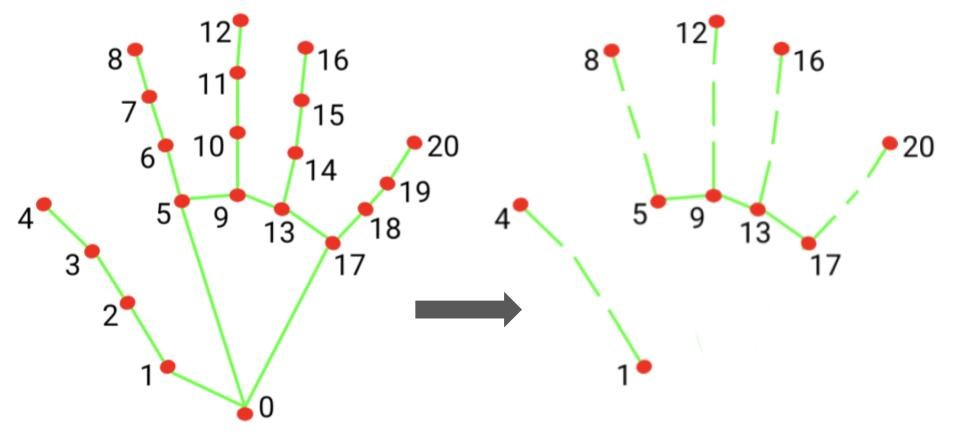
\includegraphics[width=0.95\columnwidth]{hand_keypoint_image.jpg}
\caption{Keypoint layouts considered in this study. Left: full 21-keypoint hand skeleton. Right: reduced 10-keypoint skeleton using finger bases and fingertips.}
\label{fig:keypoint_layouts}
\end{figure}

\section{LITERATURE REVIEW}.

\medskip
\noindent\textbf{Point:} The literature does not converge on a single architectural strategy for efficient pose estimation.  
\textbf{Evidence:} Existing approaches include CNN-based systems such as MediaPipe Hands~\cite{mediapipe}, attention-based models~\cite{attentionlite}, hybrid CNN-transformer designs such as EdgePose~\cite{edgepose} and temporal GCN-based tracking~\cite{handobjectgcn}.  
\textbf{Explanation:} This suggests that the literature has not yet established a single dominant architecture for achieving efficient hand-pose estimation.  
\textbf{Link:} It is reasonable to evaluate a DRHand-inspired architecture rather than assume that the design space has already been settled.

\medskip
\noindent\textbf{Point:} Edge deployment imposes a speed-accuracy tradeoff in pose estimation.  
\textbf{Evidence:} Prior work such as SPLite Hand~\cite{splitehand} shows the tradeoff and actively caters for it. while other papers assume desktop level compute.
\textbf{Explanation:} The literature therefore shows a persistent mismatch between models optimised for benchmark accuracy and models that are practical on embedded hardware.  
\textbf{Link:} This justifies treating runtime and deployment cost as core evaluation criteria

\medskip
\noindent\textbf{Point:} Lightweight pose estimation methods typically achieve efficiency through architectural, computational, and pipeline-level simplifications.  
\textbf{Evidence:} Reported strategies include compact backbones and lightweight attention~\cite{attentionlite}, sparse or reduced-complexity computation~\cite{splitehand} and detector-to-tracker pipelines with cropped regions of interest~\cite{mediapipe}.  
\textbf{Explanation:} These studies imply that efficient performance usually comes from reducing unnecessary computation across multiple stages of the model rather than from a single isolated modification.  
\textbf{Link:} This provides literature support for testing whether simpler prediction targets can preserve useful hand-pose performance.

\medskip
\noindent\textbf{Point:} The realism and domain characteristics of training data are important determinants of cross-domain generalisation in hand-pose estimation. 
\textbf{Evidence:} Prior work uses both synthetic datasets such as RHD and real datasets for hand tracking, while augmentation is often introduced to improve robustness under more realistic conditions~\cite{handobjectgcn,lightweightgcnhand,handaugment}.  
\textbf{Explanation:} These data sources differ in appearance, so a model trained on one domain may not generalise reliably to another. This is especially relevant when a study relies heavily on synthetic supervision but aims to operate on real camera input.  
\textbf{Link:} Therefore, dataset realism and cross-domain robustness remain important considerations in lightweight hand-pose estimation.

\medskip
\noindent\textbf{Point:} The literature leaves open whether full 21-keypoint hand representations are always necessary for lightweight edge-HCI use.  
\textbf{Evidence:} Existing lightweight hand-pose systems such as MediaPipe Hands~\cite{mediapipe}, Attention!~\cite{attentionlite}, and SPLite Hand~\cite{splitehand} focus mainly on reducing model complexity while still predicting a full hand structure.  
\textbf{Explanation:} This suggests that prior work has concentrated more on compressing the model than on questioning whether the full landmark target is required for practical HCI interaction.  
\textbf{Link:} This directly motivates the present study's comparison between reduced 10-keypoint and standard 21-keypoint prediction.

\medskip
These gaps motivate three main research questions:
\begin{enumerate}
    \item Is a reduced 10-keypoint representation sufficient for lightweight edge-HCI use?
    \item Does dual-branch fusion provide enough benefit to justify its added complexity?
    \item Can pseudo-labeled real-image data improve generalisation beyond synthetic-only training?
\end{enumerate}

\section{METHOD}

\subsection{Network Structure}

\noindent\textbf{Point:} The proposed model uses a shared backbone followed by two prediction branches.  
\textbf{Explanation:} The input is a resized RGB hand image, and most computation is shared before the network splits into heatmap and coordinate regression paths. Here, the term \emph{branch} refers to a task-specific prediction subnetwork attached to the shared backbone. In this architecture, the two branches are the heatmap regression branch and the coordinate regression branch. Figure~\ref{fig:network_structure} shows the overall DRHand-inspired network structure used in this study.

\begin{figure}[!p]
\centering
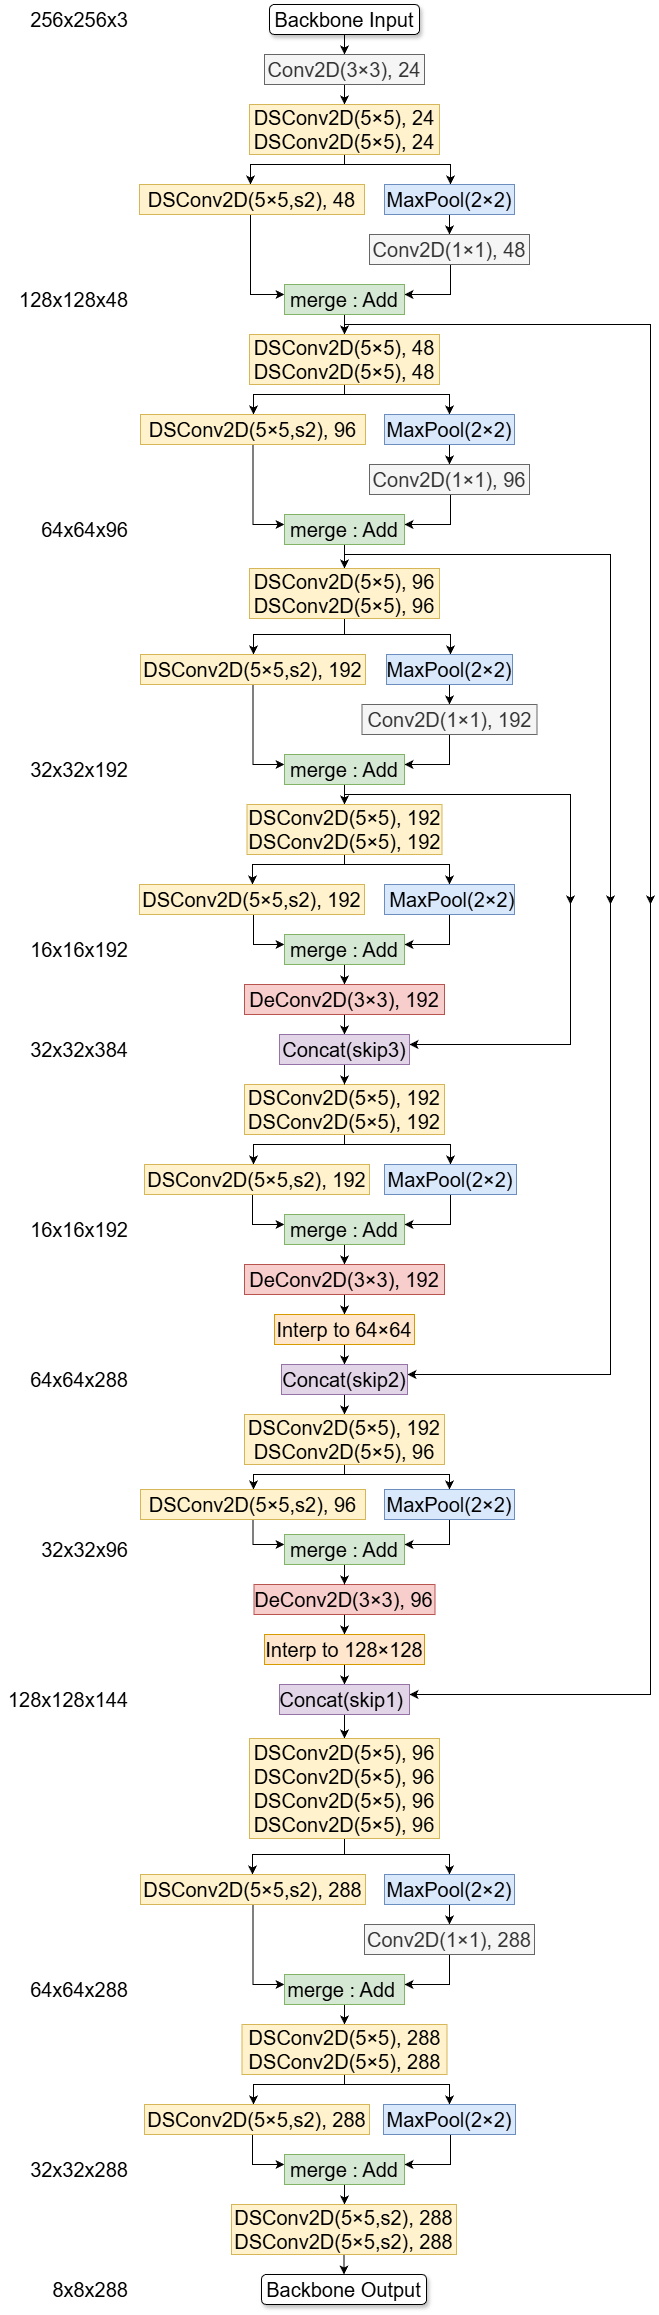
\includegraphics[width=\columnwidth,height=0.92\textheight,keepaspectratio]{4006_arch_paper-Copy of Copy of Page-7.drawio.png}
\caption{The backbone network structure.}
\label{fig:network_structure}
\end{figure}

\subsubsection{The Backbone Network}

\noindent\textbf{Point:} The backbone is designed to extract useful hand features.  
\textbf{Explanation:} Formally, the input to the model is an RGB image resized to $256 \times 256$, denoted by $x \in \mathbb{R}^{3 \times 256 \times 256}$. The backbone then produces a compact feature representation,
\begin{equation}
F = B(x).
\label{eq:backbone-features}
\end{equation}
The backbone is built from depthwise-separable convolutions, downsampling blocks, and skip-connected upsampling stages.

\subsubsection{The Heatmap Regression Branch}

\noindent\textbf{Point:} The heatmap branch predicts one spatial confidence map per keypoint.  
\textbf{Explanation:} From the shared representation, the heatmap branch predicts \(K\) output heatmaps,
\begin{equation}
\hat{H} = R_h(F).
\label{eq:heatmap-output}
\end{equation}
Here, \(K\) is the number of predicted keypoints, so \(\hat{H} \in \mathbb{R}^{K \times 64 \times 64}\) contains one \(64 \times 64\) heatmap for each keypoint. For keypoint \(i\), \(\hat{H}_i(u,v)\) denotes the predicted confidence at spatial location \((u,v)\) on the \(64 \times 64\) heatmap grid, where \(u\) and \(v\) are the horizontal and vertical heatmap indices respectively. Let \(p_i = (x_i, y_i)\) denote the ground-truth location of keypoint \(i\), expressed in the same heatmap coordinate system. The target heatmap for keypoint \(i\) is then defined as a 2D Gaussian centered at the true keypoint location,
\begin{equation}
G_i(u,v) = \exp\left(
-\frac{(u-x_i)^2 + (v-y_i)^2}{2\sigma^2}
\right),
\label{eq:gaussian-target}
\end{equation}
where \(\sigma > 0\) is the standard deviation of the Gaussian, measured in heatmap-grid units, and controls the spread of the target peak. A larger \(\sigma\) produces a broader peak, while a smaller \(\sigma\) produces a sharper target concentrated around the true landmark.

The heatmap branch is supervised using mean-squared error between the predicted heatmaps and the target heatmaps:
\begin{equation}
\mathcal{L}_{hm}
=
\frac{1}{KHW}
\sum_{i=1}^{K}
\sum_{u,v}
\left(\hat{H}_i(u,v) - G_i(u,v)\right)^2
\label{eq:heatmap-loss}
\end{equation}
Here, \(H\) and \(W\) denote the heatmap height and width. This loss averages the squared difference over all keypoints and all spatial locations, encouraging each predicted heatmap to assign a high response near the true keypoint position and a low response elsewhere. 

\subsubsection{The Coordinate Regression Branch}

\noindent\textbf{Point:} The coordinate branch predicts landmark positions directly from intermediate features.  
\textbf{Explanation:} Rather than producing a spatial heatmap for each keypoint, this branch regresses the landmark coordinates directly. It takes as input the intermediate \(64 \times 64\) feature map produced within the heatmap pathway, allowing the coordinate branch to reuse features that already encode spatial hand structure.

The coordinate branch predicts normalised landmark coordinates,
\begin{equation}
\hat{P}^{coord} = R_c(M), \qquad \hat{P}^{coord} \in \mathbb{R}^{K \times 2},
\label{eq:coord-output}
\end{equation}
where \(M\) denotes the intermediate \(64 \times 64\) feature map passed from the heatmap branch to the coordinate regressor, \(R_c(\cdot)\) denotes the coordinate-regression subnetwork, and \(K\) is the number of predicted keypoints. For keypoint \(i\), the output \(\hat{p}^{coord}_i = (\hat{x}_i, \hat{y}_i)\) represents the predicted normalised 2D coordinate, with both values expressed in the range \([0,1]\).

Let \(p_i = (x_i, y_i)\) denote the corresponding ground-truth normalised coordinate for keypoint \(i\). The coordinate branch is supervised using Wing loss,
\begin{equation}
\mathcal{L}_{coord}
=
\frac{1}{2K}
\sum_{i=1}^{K}
\sum_{j \in \{x,y\}}
\phi\!\left(\hat{p}^{coord}_{i,j} - p_{i,j}\right),
\label{eq:coord-loss}
\end{equation}
where \(\hat{p}^{coord}_{i,j}\) and \(p_{i,j}\) are the predicted and ground-truth values of the \(j\)-th coordinate component, and
\begin{equation}
\phi(\delta)=
\begin{cases}
w \ln\left(1 + \frac{|\delta|}{\epsilon}\right), & |\delta| < w, \\
|\delta| - C, & \text{otherwise,}
\end{cases}
\label{eq:wing-loss}
\end{equation}
where
\begin{equation}
C = w - w \ln\left(1 + \frac{w}{\epsilon}\right).
\end{equation}
\(\delta\) is the scalar prediction error for one coordinate value, \(w\) controls the range over which the loss behaves logarithmically, \(\epsilon\) controls the curvature near zero, and \(C\) is a constant chosen so that the piecewise function is continuous at \(|\delta| = w\).

Wing loss places greater emphasis on reducing small and medium localisation errors than standard \(L_1\) or \(L_2\) losses, while remaining less sensitive to very large errors.

\begin{figure}[H]
\centering
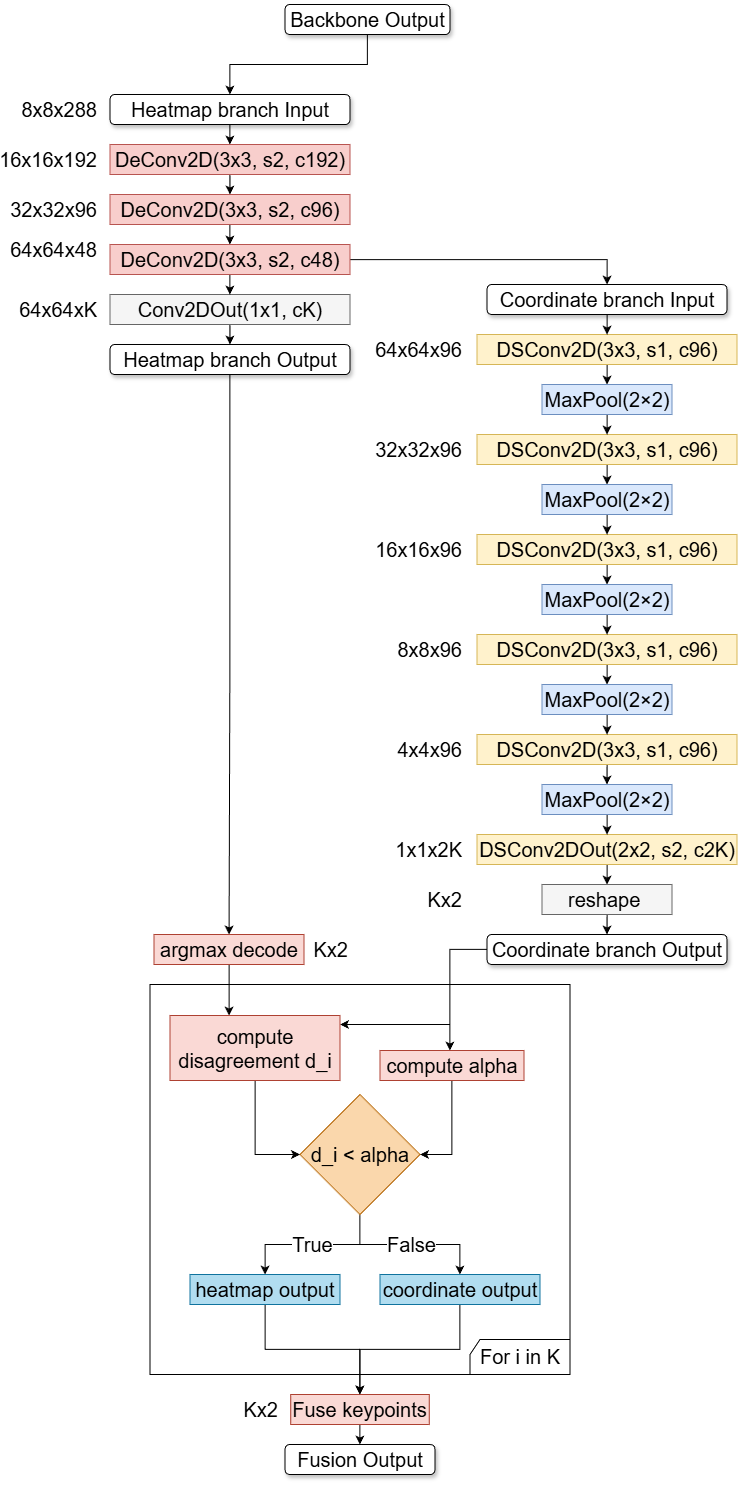
\includegraphics[width=\columnwidth,height=0.60\textheight,keepaspectratio]{4006_arch_paper-hm_c_f.drawio.png}
\caption{The heatmap, coordinate, and fusion components.}
\label{fig:hm_coord_fusion}
\end{figure}

\subsection{Post Processing}

\noindent\textbf{Point:} The final pose can be produced by either branch alone or by a simple fusion rule.  
\textbf{Explanation:} The implementation supports three inference modes: heatmap-only, coordinate-only, and fusion. In heatmap-only mode, landmark locations are obtained by decoding the peak of each predicted heatmap. In coordinate-only mode, the direct regression output is used as the final pose. In fusion mode, the two predictions are compared joint-by-joint and a simple heuristic selects which branch to trust for each landmark.

At inference time, let \(\hat{H}_i\) denote the predicted heatmap for keypoint \(i\), with spatial dimensions \(H \times W\). The heatmap-based prediction is obtained by taking the spatial argmax,
\begin{equation}
(u_i^*, v_i^*) = \arg\max_{u,v} \hat{H}_i(u,v),
\label{eq:heatmap-argmax}
\end{equation}
where \((u_i^*, v_i^*)\) is the location of the peak response on the discrete heatmap grid. This peak is then converted into normalized image coordinates,
\begin{equation}
\hat{p}^{hm}_i =
\left(
\frac{u_i^*}{W-1},
\frac{v_i^*}{H-1}
\right).
\label{eq:heatmap-decode}
\end{equation}
The coordinate branch directly predicts the normalized coordinate \(\hat{p}^{coord}_i\) for the same joint, so both outputs lie in the same \([0,1]\) coordinate space and can be compared directly.

For each joint \(i\), the disagreement between the two branches is measured by Euclidean distance,
\begin{equation}
d_i = \left\| \hat{p}^{hm}_i - \hat{p}^{coord}_i \right\|_2.
\label{eq:fusion-disagreement}
\end{equation}
A sample-specific threshold \(\alpha\) is then computed from the coordinate-branch output as the median predicted bone length,
\begin{equation}
\alpha = \mathrm{median}_{(a,b)\in \mathcal{E}}
\left\| \hat{p}^{coord}_a - \hat{p}^{coord}_b \right\|_2,
\label{eq:fusion-threshold}
\end{equation}
where \(\mathcal{E}\) denotes the set of hand-skeleton edges. \(\alpha\) acts as a scale-adaptive tolerance: for a larger predicted hand, a larger disagreement between the two branches may still be acceptable, whereas for a smaller predicted hand, the same disagreement would be more significant.

The fused output for joint \(i\) is defined as
\begin{equation}
\hat{p}^{fused}_i =
\begin{cases}
\hat{p}^{hm}_i, & d_i < \alpha, \\
\hat{p}^{coord}_i, & \text{otherwise.}
\end{cases}
\label{eq:fused-output}
\end{equation}
Thus, fusion is performed independently for each joint. When the two branches agree closely, the heatmap-decoded prediction is used; otherwise, the coordinate-regression prediction is retained.

\section{EXPERIMENTS}

\subsection{Datasets}

The Rendered Handpose Dataset (RHD)~\cite{rhd} is used as the main synthetic benchmark in this study. It provides 41,258 training samples and 2,728 testing samples. Each sample contains a Blender rendered $320 \times 320$ RGB hand image, and 21 hand keypoints with image-space coordinates and visibility labels. the standard training/evaluation split is used.

The second dataset is HK26K (Kaggle)~\cite{hk26k}, is the more realistic image domain for transfer learning. 18,776 training images and 7,992 validation images. The images are drawn from hand-photo and gesture datasets such as 11K Hands~\cite{hands11k}, 2000 Hand Gestures~\cite{giridhar_hand_gestures}, and the Gesture Recognition Dataset~\cite{gesture_recognition_kaggle}, and include both hand-only views and realistic photographed scenes. the annotations are generated using MediaPipe and act as pseudo-labels. the standard training/evaluation split is used.

A pre-defined subset of an 8-image real-hand evaluation set (RH8) is also used for evaluation. This set contains 8 original real RGB hand images showing basic single-hand gestures on a white background, with annotations initialized from MediaPipe predictions and then manually corrected.

\subsection{Implementation Details}

The proposed network was implemented in PyTorch and trained on an NVIDIA Tesla A100 80GB GPU, hosted on Kelvin2 HPC, using the Adam optimizer. Two output configurations were used in this study: a standard 21-keypoint model and a reduced 10-keypoint variant. In both cases, the same overall architecture was retained, with only the output dimensionality of the prediction heads changed. Training followed a two-stage procedure. In stage 1, only the backbone and heatmap branch were optimized with learning rate \(10^{-3}\) and batch size 64. In stage 2, the coordinate branch was added and the model was further optimized with learning rate \(10^{-4}\) and an effective batch size of 256, implemented as batch size 64 with gradient accumulation. Runtime benchmarking for deployment-oriented evaluation was performed separately on Jetson Orin Nano 8GB, using its embedded Ampere GPU.

\subsection{Differences in this implementation and DRHand}

\noindent This repository is a DRHand-inspired implementation rather than a strict reproduction of the original paper. The original work was implemented in TensorFlow and trained on YouTube2D Hands and GANerated Hands, whereas the present study is implemented in PyTorch and focuses on RHD together with pseudo-labeled HK26K data. Some optimisation details were not fully specified in the original paper, so several training values had to be reconstructed in this implementation. The reported results should therefore be interpreted as evidence about this reconstructed DRHand-style pipeline rather than as a direct numerical replication of the original study.


\subsection{Evaluation Metrics}

\noindent\textbf{Point:} Three main pose-estimation metrics are used to evaluate prediction quality.  
\textbf{Explanation:} The learned models are evaluated using sum of squared error (SSE), end-point error (EPE), and probability of correct keypoint (PCK). Let \(p_{si}, \hat{p}_{si} \in [0,1]^2\) denote the ground-truth and predicted normalized 2D coordinates of keypoint \(i\) in sample \(s\), and let \(v_{si} \in \{0,1\}\) denote a visibility mask, where \(v_{si}=1\) if the evaluated keypoint is visible and \(v_{si}=0\) otherwise. Thus, invisible keypoints do not contribute to the reported error values. All distances below are Euclidean distances in normalized coordinate space.

The normalised SSE is defined as
\begin{equation}
\mathrm{SSE} =
\frac{1}{N}
\sum_{s=1}^{N}
\sum_{i=1}^{K}
v_{si}\left\|
\hat{p}_{si} - p_{si}
\right\|_2^2,
\label{eq:sse}
\end{equation}
where \(N\) is the number of samples and \(K\) is the number of evaluated keypoints. This metric sums the squared localization error over all visible evaluated keypoints in each sample and then averages that total over the dataset. Lower SSE therefore indicates lower overall pose error.

\medskip
\noindent\textbf{Point:} End-point error is measured in a root-relative normalized form.  
\textbf{Explanation:} EPE is computed after subtracting a designated root joint from both the prediction and the ground truth. This removes global translation and measures how well the relative hand structure is recovered. Let \(r\) denote the root keypoint used for the current evaluation layout. In the full layout, keypoint \(0\) is used when available. In reduced or shared-10 evaluation, keypoint \(1\) is used when keypoint \(0\) is absent, as shown in Figure~\ref{fig:keypoint_layouts}.

The normalized root-relative EPE is defined as
\begin{equation}
\mathrm{EPE} =
\frac{
\sum_{s=1}^{N}
\sum_{i=1}^{K}
v_{si}
\left\|
(\hat{p}_{si} - \hat{p}_{sr}) - (p_{si} - p_{sr})
\right\|_2
}{
\sum_{s=1}^{N}
\sum_{i=1}^{K}
v_{si}
},
\label{eq:epe}
\end{equation}
where \(\hat{p}_{sr}\) and \(p_{sr}\) are the predicted and ground-truth coordinates of the root keypoint in sample \(s\). This metric reports the mean visible-joint distance after root alignment, so lower EPE indicates better recovery of the relative pose configuration. EPE is reported only when a supported root keypoint is present in the evaluated layout.

\medskip
\noindent\textbf{Point:} PCK measures the proportion of visible keypoints localized within a fixed error threshold.  
\textbf{Explanation:} In this study, a keypoint is counted as correct when its normalized distance from the ground truth is at most \(0.2\). This threshold is retained from the original DRHand evaluation protocol. Higher PCK therefore indicates a larger fraction of acceptable landmark predictions under the same tolerance.

\begin{equation}
\mathrm{PCK}_{\sigma} =
\frac{
\sum_{s=1}^{N}
\sum_{i=1}^{K}
v_{si}\,\mathbf{1}
\left(
\left\|
\hat{p}_{si} - p_{si}
\right\|_2 \le \sigma
\right)
}{
\sum_{s=1}^{N}
\sum_{i=1}^{K}
v_{si}
},
\qquad \sigma = 0.2,
\label{eq:pck}
\end{equation}
where \(\mathbf{1}(\cdot)\) is the indicator function, which returns \(1\) when the condition is true and \(0\) otherwise. Thus, PCK is the fraction of visible evaluated keypoints whose localization error falls within the accepted threshold. In this evaluation section, \(\sigma\) denotes the PCK threshold.

\medskip
\noindent\textbf{Point:} Runtime is reported separately from pose accuracy.  
\textbf{Explanation:} Deployment-oriented evaluation includes prediction time in milliseconds per image and throughput in images per second. For the Jetson measurements, both forward-only and end-to-end timings are reported to distinguish model computation from surrounding pipeline overhead.

\medskip
\noindent\textbf{Point:} Additional metrics are used for baseline and fusion-specific analysis.  
\textbf{Explanation:} For the MediaPipe baseline, detection success rate is reported because the pipeline may fail before landmark prediction. For fusion analysis, the study also reports how often the heatmap branch or the coordinate branch is selected, how strongly their predictions disagree, the typical size of the adaptive fusion threshold, and how often the heuristic agrees with an oracle choice of the lower-error branch computed using ground truth.

Let \(m_{si} \in \{0,1\}\) denote the branch-selection decision for keypoint \(i\) in sample \(s\), where \(m_{si}=1\) if fusion selects the heatmap prediction and \(m_{si}=0\) if fusion selects the coordinate-regression prediction. The heatmap-selection and coordinate-selection rates are then
\begin{equation}
\mathrm{Sel}^{hm} =
\frac{1}{NK}
\sum_{s=1}^{N}\sum_{i=1}^{K} m_{si},
\qquad
\mathrm{Sel}^{coord} =
\frac{1}{NK}
\sum_{s=1}^{N}\sum_{i=1}^{K} (1-m_{si}).
\label{eq:selection-rates}
\end{equation}
These rates describe how often each branch contributes the final fused output across all evaluated joints.
The reported fusion-threshold statistics are the mean and median of \(\alpha_s\) over all evaluated samples. Intuitively, \(\alpha_s\) reflects the predicted hand scale for that sample and determines how much disagreement between branches is tolerated before the coordinate branch is preferred.

An oracle branch label is defined for each visible evaluated keypoint by comparing the two branch errors directly against ground truth:
\begin{equation}
o_{si} =
\mathbf{1}
\left(
\left\|
\hat{p}^{hm}_{si} - p_{si}
\right\|_2
\le
\left\|
\hat{p}^{coord}_{si} - p_{si}
\right\|_2
\right).
\label{eq:oracle-label}
\end{equation}
The oracle-match rate is then
\begin{equation}
\mathrm{OracleMatch} =
\frac{
\sum_{s=1}^{N}\sum_{i=1}^{K}
v_{si}\,\mathbf{1}(m_{si}=o_{si})
}{
\sum_{s=1}^{N}\sum_{i=1}^{K} v_{si}
}.
\label{eq:oracle-match}
\end{equation}
This metric reports how often the fusion heuristic selected the lower-error branch on visible evaluated keypoints. A higher oracle-match rate therefore indicates that the fusion rule more often makes the locally correct decision.
Each learned-model configuration was trained and evaluated in five independent runs using different random seeds. Reported values for learned models are therefore given as mean \(\pm\) standard deviation across those five runs.

\section{RESULTS AND ANALYSIS}

\subsection{Experimental Results}

The learned-model configurations are as follows: the standard 21-keypoint baseline is referred to as Baseline-21, the reduced 10-keypoint model as Reduced-10, the single-domain transfer baselines as RHD-only and HK26K-only, and the fine-tuned transfer models as HK26K$\rightarrow$RHD and RHD$\rightarrow$HK26K.

\subsubsection{Reduced Keypoint Performance}

\noindent\textbf{Point:} The reduced 10-keypoint model retains broadly comparable performance to the 21-keypoint baseline on the shared subset.  
\textbf{Evidence:} In Table~\ref{tab:main_accuracy}, the shared-10 evaluation of Baseline-21 gives SSE 0.1511, EPE 0.0764, and PCK 0.9101, while the native-10 Reduced-10 model gives SSE 0.1574, EPE 0.0706, and PCK 0.9099.  
\textbf{Explanation:} These values are very close, indicating that reducing the landmark set does not substantially weaken performance on the subset of keypoints most relevant to the reduced representation.  
\textbf{Link:} This supports the claim that a smaller landmark set can remain viable for lightweight edge-HCI use.

\subsubsection{Runtime and Deployment Cost}

\medskip
\noindent\textbf{Point:} The runtime advantage of the 10-keypoint model appears mainly in fusion mode.  
\textbf{Evidence:} In Tables~\ref{tab:latency} and~\ref{tab:latency_breakdown}, the forward-time gap between Baseline-21 and Reduced-10 is much larger in fusion mode (27.43 vs 24.59 ms/image) than in heatmap mode (24.28 vs 24.00 ms/image) or coordinate mode (24.08 vs 23.91 ms/image). The detailed breakdown further shows that the largest difference appears in the forward stage, while the surrounding pipeline costs are comparatively similar.  
\textbf{Explanation:} Since the single-branch modes differ only slightly, the main efficiency gain of the reduced model appears to come from lower fusion-stage overhead rather than from a large reduction in shared network cost.  
\textbf{Link:} This suggests that the practical speed benefit of the 10-keypoint model is tied mainly to the post-processing stage. The minor yet consistent speed gains seen with single branch results prompt further investigation. 

\subsubsection{Branch Behaviour}

\medskip
\noindent\textbf{Point:} Fusion provides the strongest overall balance of branch behaviour.  
\textbf{Evidence:} In Table~\ref{tab:branch_ablation}, fusion gives the lowest SSE and EPE for both Baseline-21 and Reduced-10, while maintaining PCK values that remain close to the best single-branch result. For Baseline-21, heatmap-only achieves the highest PCK but at the cost of substantially worse EPE, whereas for Reduced-10, coordinate-only gives only a marginal PCK gain over fusion while fusion retains better SSE and EPE.  
\textbf{Explanation:} This suggests that the two branches contribute complementary strengths: the heatmap branch can improve threshold-based correctness, while the coordinate branch preserves stronger geometric structure. Fusion provides the most balanced overall operating point across these error criteria.  
\textbf{Link:} Accordingly, the branch-ablation results support the use of fusion as the main operating mode of the system.

\subsubsection{Transfer and Real-Image Adaptation}

\medskip
\noindent\textbf{Point:} The experiments show that synthetic-only training does not generalize reliably to more realistic image domains, but pseudo-labeled real-image supervision provides a useful adaptation bridge.  
\textbf{Evidence:} In Table~\ref{tab:transfer_learning}, the RHD-trained model performs strongly on RHD but poorly on HK26K, while the HK26K-trained model shows the opposite pattern. After target-domain adaptation, RHD$\rightarrow$HK26K and HK26K$\rightarrow$RHD both improve substantially over their cross-domain starting points. This interpretation is further supported by the small real-image benchmark in Table~\ref{tab:hand_frame_small_pilot}, where the HK26K-oriented models, especially HK26K-only and RHD$\rightarrow$HK26K, perform more strongly than the RHD-only baselines.  
\textbf{Explanation:} These results suggest that the main difficulty is the domain gap between synthetic training data and more realistic image conditions. Pseudo-labeled real-image data does not provide perfect supervision, but it appears to move the model closer to the real-image domain than synthetic-only training can achieve on its own.  
\textbf{Link:} Therefore, the transfer results are best interpreted as evidence that pseudo-labeled real-image supervision can act as a practical adaptation bridge beyond synthetic-only training.

\medskip
\noindent\textbf{Point:} A small real-image benchmark was also included.  
\textbf{Explanation:} In addition to the main benchmark results on RHD and HK26K, the models were evaluated on RH8, which contains eight real images with annotations initialized from MediaPipe predictions and then manually corrected. These results provide a small but explicit real-image benchmark alongside the larger synthetic and pseudo-labeled datasets.

\subsubsection{Fusion Diagnostics}

\medskip
\noindent\textbf{Point:} The current fusion heuristic is useful but clearly imperfect.  
\textbf{Evidence:} In Table~\ref{tab:fusion_diagnostics}, the oracle-match rate is only about 0.48 for Baseline-21 and 0.53 for Reduced-10, even though fusion improves aggregate accuracy in the branch-ablation study.  
\textbf{Explanation:} This means that the heuristic often fails to choose the lower-error branch on a per-joint basis, but still helps overall because some of its correct decisions occur on more influential prediction cases.  
\textbf{Link:} Therefore, the current fusion rule is beneficial, but it also remains one of the clearest opportunities for future improvement.

\subsubsection{Hyperparameter Sensitivity}

\medskip
\noindent\textbf{Point:} The baseline hyperparameter setting is a compromise rather than an obviously dominant configuration.  
\textbf{Evidence:} In Table~\ref{tab:hyper_ablation}, several alternative settings improve one metric while worsening another; for example, \texttt{E1} improves EPE and PCK relative to Baseline-21, whereas \texttt{W2} gives the lowest SSE, but no single configuration is uniformly best across all reported metrics.  
\textbf{Explanation:} The hyperparameter study suggests that not all settings matter equally. The end-to-end runtime changes are small across all variants, so these hyperparameters have negligible effect on deployment cost. In contrast, accuracy is more sensitive to some parameters than others. The Wing-loss parameter \(\epsilon\) appears particularly influential: \texttt{E1} improves EPE and PCK relative to the baseline, whereas \texttt{E2} noticeably worsens EPE. The heatmap width \(\sigma\) and the Wing-loss parameter \(w\) also affect the accuracy tradeoff, but in a more mixed way, with some variants improving SSE, EPE, or PCK at the expense of others. By comparison, the loss-weight variants mainly produce smaller or less consistently beneficial changes, aside from \texttt{L1}, which degrades SSE. Overall, the baseline should therefore be viewed as a practical compromise, while \(\epsilon\) appears to be the most influential of the tested hyperparameters.  
\textbf{Link:} As a result, the hyperparameter study suggests that the selected baseline is a reasonable compromise rather than a clearly dominated operating point.

\subsection{Qualitative Results}

\subsubsection{Real-Image Behaviour}

\medskip
\noindent\textbf{Point:} The real-image examples favour the HK26K-oriented models.  
\textbf{Evidence:} In the two RH8 figures, HK26K-only and especially RHD$\rightarrow$HK26K place the red landmarks closer to the green annotations than Baseline-21 and Reduced-10, particularly around the inner finger cluster.  
\textbf{Explanation:} This suggests that the real-image examples are visually closer to the HK26K domain than to the synthetic RHD domain.  
\textbf{Link:} The qualitative results therefore support the transfer findings on real-image adaptation.

\subsubsection{Cross-Dataset Failure and Adaptation}

\medskip
\noindent\textbf{Point:} The model trained only on HK26K generalizes poorly when evaluated on the RHD dataset.  
\textbf{Evidence:} In the RHD examples \texttt{00143} and \texttt{00354}, the HK26K-only model produces landmark groups that are visibly detached from the hand.  
\textbf{Explanation:} This is a clear visual failure under cross-dataset domain shift rather than a minor local error.  
\textbf{Link:} The selected figures therefore reinforce the conclusion that zero-shot transfer from HK26K to RHD is weak.

\medskip
\noindent\textbf{Point:} Target-domain adaptation improves the transferred HK26K model on RHD.  
\textbf{Evidence:} In \texttt{00354}, HK26K$\rightarrow$RHD is visibly better aligned to the hand than HK26K-only, even though it is not the strongest prediction in the figure.  
\textbf{Explanation:} Fine-tuning reduces the most obvious cross-domain failures, but does not eliminate them completely.  
\textbf{Link:} This supports the interpretation that transfer is useful mainly as initialization for later target-domain adaptation.

\medskip
\noindent\textbf{Point:} RHD$\rightarrow$HK26K is the most consistently strong learned model across the selected figures.  
\textbf{Evidence:} In Figures~\ref{fig:qual_real_1} and~\ref{fig:qual_real_2}, RHD$\rightarrow$HK26K is among the closest predictions to the ground truth on the two real-image examples, and in Figures~\ref{fig:qual_rhd_1} and~\ref{fig:qual_rhd_2} it remains stable on the two RHD examples, unlike HK26K-only. This visual pattern is also consistent with the quantitative transfer results in Table~\ref{tab:transfer_learning}.  
\textbf{Explanation:} This indicates that RHD pretraining followed by HK26K adaptation transfers more consistently across the displayed cases than HK26K-only training.  
\textbf{Link:} The selected figures therefore visually support the transfer asymmetry seen in the quantitative results.

\subsubsection{MediaPipe Comparison Caveat}

\medskip
\noindent\textbf{Point:} In Figures~\ref{fig:qual_real_1} and~\ref{fig:qual_real_2}, MediaPipe is visually strong, but the real-image comparison is not fully independent.
\textbf{Evidence:} MediaPipe aligns closely with the annotations in the two RH8 figures, but those annotations were initialized from MediaPipe predictions before manual correction.  
\textbf{Explanation:} This gives MediaPipe a structural advantage on that small benchmark set.  
\textbf{Link:} The real-image MediaPipe comparisons should therefore be treated as illustrative rather than definitive.

\section{CONCLUSION AND FUTURE WORK}

\noindent\textbf{Point:} A reduced 10-keypoint representation is sufficient for the lightweight edge-HCI setting studied here.
\textbf{Evidence:} The reduced model remains close to the baseline in predictive quality while offering a runtime advantage.
\textbf{Explanation:} This shows that the full 21-keypoint output is not strictly necessary for the interaction-focused scope of this study.
\textbf{Link:} The first research question is answered positively.

\medskip
\noindent\textbf{Point:} Dual-branch fusion is justified, but only as a marginal improvement with minimal time expense.
\textbf{Evidence:} Fusion gives the best overall balance across the reported results, but the diagnostic analysis shows that the current selection rule is not fully optimal.
\textbf{Explanation:} The two-branch design is useful, yet the present heuristic does not extract all of its potential benefit.
\textbf{Link:} The second research question is answered as a qualified yes.

\medskip
\noindent\textbf{Point:} Pseudo-labeled real-image data improves generalisation beyond synthetic-only training, especially when used for target-domain adaptation.
\textbf{Evidence:} The transfer results show that zero-shot cross-domain generalisation is weak, but fine-tuning on the target domain substantially improves performance.
\textbf{Explanation:} This means pseudo-labeled real-image supervision is helpful, but mainly as an adaptation mechanism rather than as a complete replacement for target-domain training.
\textbf{Link:} The third research question is also answered positively, with that limitation.

\medskip
\noindent\textbf{Point:} Future work should redesign the architecture specifically for reduced 10-keypoint prediction.
\textbf{Evidence:} The current results show that the reduced target remains effective, but the model still follows essentially the same DRHand-inspired design as the 21-keypoint version.
\textbf{Explanation:} A purpose-built reduced architecture may allow further reductions in model size and latency.
\textbf{Link:} The next step is therefore to test whether a smaller model can preserve the same practical accuracy in the 10-keypoint setting.

\medskip
\noindent\textbf{Point:} Real-image evaluation should be broadened beyond the current pilot set.
\textbf{Evidence:} The present study includes only a small manually annotated real-image dataset used for supplementary quantitative and qualitative comparison.
\textbf{Explanation:} A larger independently annotated real-image benchmark is needed to assess practical robustness more convincingly.
\textbf{Link:} Future work should therefore prioritise broader real-world evaluation.

\medskip
\noindent\textbf{Point:} Fusion remains one of the clearest opportunities for improvement.
\textbf{Evidence:} The current diagnostics show that the heuristic often fails to select the lower-error branch, and the original DRHand formulation also leaves room for stronger branch combination~\cite{dualreg}.
\textbf{Explanation:} A more principled or learned fusion strategy could improve both robustness and accuracy.
\textbf{Link:} Future work should therefore investigate improved fusion design.

\medskip
\noindent\textbf{Point:} Future work should introduce an explicit hand-detection stage to standardise the hand input before pose estimation.
\textbf{Evidence:} The current learned pipeline assumes a prepared hand region, while practical systems such as MediaPipe first localise the hand and then estimate landmarks from a normalized crop.
\textbf{Explanation:} A detection stage could produce more consistent hand scale, position, and framing, making the pose input distribution closer to the data seen during training and reducing reliance on aggressive spatial augmentation.
\textbf{Link:} Future work should therefore evaluate whether detector-based input normalisation improves robustness and simplifies the pose-learning stage.

\clearpage
\onecolumn
\section*{TABLES}

\begin{table}[H]
\centering
\footnotesize
\caption{Main quantitative comparison between the 21-keypoint baseline and the reduced 10-keypoint model on RHD. Lower SSE and EPE are better; higher PCK@0.2 is better. Values are mean $\pm$ std over five seeds.}
\label{tab:main_accuracy}
\begin{tabular}{llcccc}
\toprule
Model & Eval set & Train joints & SSE $\downarrow$ & EPE $\downarrow$ & PCK@0.2 $\uparrow$ \\
\midrule
Baseline-21 & native-21 & 21 & 0.3098 $\pm$ 0.0236 & 0.0779 $\pm$ 0.0054 & 0.9112 $\pm$ 0.0071 \\
Baseline-21 & shared-10 & 21 & 0.1511 $\pm$ 0.0120 & 0.0764 $\pm$ 0.0039 & 0.9101 $\pm$ 0.0071 \\
Reduced-10 & native-10 & 10 & 0.1574 $\pm$ 0.0226 & 0.0706 $\pm$ 0.0054 & 0.9099 $\pm$ 0.0046 \\
\bottomrule
\end{tabular}
\end{table}

\begin{table}[H]
\centering
\footnotesize
\caption{Edge-device latency summary for the main models. Forward time measures the prediction stage only, whereas end-to-end time includes image read, preprocessing, host-to-device transfer, prediction, and JSON write. Values are mean $\pm$ std over five seeds.}
\label{tab:latency}
\begin{tabular}{llccc}
\toprule
Model & Mode & Forward ms/img $\downarrow$ & End-to-end ms/img $\downarrow$ & Images/s $\uparrow$ \\
\midrule
Baseline-21 & fusion & 27.43 $\pm$ 0.45 & 36.81 $\pm$ 1.33 & 27.20 $\pm$ 0.97 \\
Baseline-21 & heatmap & 24.28 $\pm$ 0.35 & 33.19 $\pm$ 0.56 & 30.13 $\pm$ 0.50 \\
Baseline-21 & coord & 24.08 $\pm$ 0.44 & 33.17 $\pm$ 0.86 & 30.16 $\pm$ 0.77 \\
Reduced-10 & fusion & 24.59 $\pm$ 0.61 & 33.31 $\pm$ 0.71 & 30.03 $\pm$ 0.64 \\
Reduced-10 & heatmap & 24.00 $\pm$ 0.34 & 32.64 $\pm$ 0.46 & 30.64 $\pm$ 0.43 \\
Reduced-10 & coord & 23.91 $\pm$ 0.29 & 32.50 $\pm$ 0.34 & 30.77 $\pm$ 0.32 \\
\bottomrule
\end{tabular}
\end{table}

\begin{table}[H]
\centering
\footnotesize
\caption{Detailed latency breakdown for the main fused models. These metrics are available from the benchmark pipeline and help localize where runtime is spent. Values are mean $\pm$ std over five seeds.}
\label{tab:latency_breakdown}
\begin{tabular}{lcccccc}
\toprule
Model & Read ms & Prep ms & H2D ms & Forward ms & Write ms & E2E ms \\
\midrule
Baseline-21 fusion & 4.89 $\pm$ 0.64 & 2.80 $\pm$ 0.13 & 0.32 $\pm$ 0.02 & 27.43 $\pm$ 0.45 & 0.67 $\pm$ 0.09 & 36.81 $\pm$ 1.33 \\
Reduced-10 fusion & 4.49 $\pm$ 0.08 & 2.74 $\pm$ 0.05 & 0.31 $\pm$ 0.01 & 24.59 $\pm$ 0.61 & 0.52 $\pm$ 0.02 & 33.31 $\pm$ 0.71 \\
\bottomrule
\end{tabular}
\end{table}

\begin{table}[H]
\centering
\footnotesize
\caption{Branch ablation for the dual-regression design. Fusion is compared against the heatmap-only and coordinate-only outputs using the same trained checkpoints. Values are mean $\pm$ std over five seeds.}
\label{tab:branch_ablation}
\begin{tabular}{llcccc}
\toprule
Model & Eval set & Mode & SSE $\downarrow$ & EPE $\downarrow$ & PCK@0.2 $\uparrow$ \\
\midrule
Baseline-21 & native-21 & fusion & 0.3098 $\pm$ 0.0236 & 0.0779 $\pm$ 0.0054 & 0.9112 $\pm$ 0.0071 \\
Baseline-21 & native-21 & heatmap & 0.3139 $\pm$ 0.0684 & 0.0989 $\pm$ 0.0335 & 0.9374 $\pm$ 0.0066 \\
Baseline-21 & native-21 & coord & 0.3134 $\pm$ 0.0229 & 0.0788 $\pm$ 0.0062 & 0.9113 $\pm$ 0.0071 \\
Reduced-10 & native-10 & fusion & 0.1574 $\pm$ 0.0226 & 0.0706 $\pm$ 0.0054 & 0.9099 $\pm$ 0.0046 \\
Reduced-10 & native-10 & heatmap & 0.2213 $\pm$ 0.0880 & 0.0991 $\pm$ 0.0288 & 0.9022 $\pm$ 0.0393 \\
Reduced-10 & native-10 & coord & 0.1599 $\pm$ 0.0218 & 0.0715 $\pm$ 0.0070 & 0.9102 $\pm$ 0.0048 \\
\bottomrule
\end{tabular}
\end{table}

\begin{table}[H]
\centering
\footnotesize
\caption{Transfer-learning results for the four training sequences evaluated on both RHD and HK26K. Where C... refers to the COCO annotation of HK26K and is used as a shorthand. Values are mean $\pm$ std over five seeds, and fusion-mode evaluation is shown.}
\label{tab:transfer_learning}
\resizebox{\textwidth}{!}{%
\begin{tabular}{llcccccc}
\toprule
Training sequence & ID & RHD SSE & RHD EPE & RHD PCK & HK26K SSE & HK26K EPE & HK26K PCK \\
\midrule
RHD-only & \texttt{R\_ONLY} & 0.3091 $\pm$ 0.0269 & 0.0764 $\pm$ 0.0030 & 0.9143 $\pm$ 0.0097 & 3.7488 $\pm$ 0.7985 & 0.3365 $\pm$ 0.0075 & 0.3719 $\pm$ 0.0434 \\
HK26K-only & \texttt{C\_ONLY} & 1.4194 $\pm$ 0.2619 & 0.1609 $\pm$ 0.0207 & 0.3397 $\pm$ 0.0718 & 0.0764 $\pm$ 0.0016 & 0.0612 $\pm$ 0.0049 & 0.9834 $\pm$ 0.0007 \\
HK26K $\rightarrow$ RHD & \texttt{C\_TO\_R} & 0.4504 $\pm$ 0.0162 & 0.1020 $\pm$ 0.0039 & 0.8190 $\pm$ 0.0114 & 1.6426 $\pm$ 0.2293 & 0.2678 $\pm$ 0.0114 & 0.5320 $\pm$ 0.0164 \\
RHD $\rightarrow$ HK26K & \texttt{R\_TO\_C} & 0.5699 $\pm$ 0.0592 & 0.1276 $\pm$ 0.0149 & 0.7690 $\pm$ 0.0221 & 0.0980 $\pm$ 0.0064 & 0.0840 $\pm$ 0.0018 & 0.9837 $\pm$ 0.0007 \\
\bottomrule
\end{tabular}
}
\end{table}

\begin{table}[H]
\centering
\footnotesize
\caption{Real-image benchmark evaluation on RH8, the 8-image real-hand evaluation set ($n=8$ images). The annotations were initialized from MediaPipe predictions and then manually corrected. Learned-model rows are mean $\pm$ std over five seeds; MediaPipe is a single run. All learned-model results use fusion-mode evaluation.}
\label{tab:hand_frame_small_pilot}
\begin{tabular}{llcccc}
\toprule
Method & Eval protocol & SSE $\downarrow$ & EPE $\downarrow$ & PCK@0.2 $\uparrow$ & Detect. succ. \\
\midrule
Baseline-21 & shared-10 & 0.3345 $\pm$ 0.0221 & 0.2815 $\pm$ 0.0129 & 0.7075 $\pm$ 0.0143 & n/a \\
Reduced-10 & native-10 & 0.4350 $\pm$ 0.1153 & 0.2752 $\pm$ 0.0307 & 0.6475 $\pm$ 0.0555 & n/a \\
RHD-only & shared-10 & 0.3595 $\pm$ 0.0475 & 0.2706 $\pm$ 0.0214 & 0.7050 $\pm$ 0.0338 & n/a \\
HK26K-only & shared-10 & 0.1215 $\pm$ 0.0434 & 0.1155 $\pm$ 0.0286 & 0.9200 $\pm$ 0.0647 & n/a \\
HK26K$\rightarrow$RHD & shared-10 & 0.3644 $\pm$ 0.0360 & 0.2481 $\pm$ 0.0090 & 0.7075 $\pm$ 0.0301 & n/a \\
RHD$\rightarrow$HK26K & shared-10 & 0.1209 $\pm$ 0.0236 & 0.1043 $\pm$ 0.0151 & 0.9425 $\pm$ 0.0301 & n/a \\
MediaPipe & native-21 & 0.0012 & 0.0018 & 1.0000 & 1.0000 \\
MediaPipe & shared-10 & 0.0005 & 0.0017 & 1.0000 & 1.0000 \\
\bottomrule
\end{tabular}
\end{table}

\begin{table}[H]
\centering
\footnotesize
\caption{Comparison between the MediaPipe Hand Landmarker baseline and the learned DRHand variants on RHD. The MediaPipe rows are single evaluation runs using \texttt{--hand auto}, whereas the DRHand rows are mean $\pm$ std over five seeds. Detection success is shown only for the MediaPipe runs because the learned-model evaluations do not use the same detection stage.}
\label{tab:mediapipe_baseline}
\begin{tabular}{llcccc}
\toprule
Method & Eval set & SSE & EPE & PCK@0.2 & Detect. succ. \\
\midrule
MediaPipe & native-21 & 1.7049 & 0.0833 & 0.7707 & 0.8933 \\
MediaPipe & shared-10 & 0.8599 & 0.1378 & 0.7635 & 0.8933 \\
Baseline-21 fusion & native-21 & 0.3098 $\pm$ 0.0236 & 0.0779 $\pm$ 0.0054 & 0.9112 $\pm$ 0.0071 & n/a \\
Baseline-21 fusion & shared-10 & 0.1511 $\pm$ 0.0120 & 0.0764 $\pm$ 0.0039 & 0.9101 $\pm$ 0.0071 & n/a \\
Reduced-10 fusion & native-10 & 0.1574 $\pm$ 0.0226 & 0.0706 $\pm$ 0.0054 & 0.9099 $\pm$ 0.0046 & n/a \\
\bottomrule
\end{tabular}
\end{table}

\begin{table}[H]
\centering
\footnotesize
\caption{Fusion diagnostics for the dual-regression post-processing rule. The oracle-match rate measures how often the final fusion choice matches the lower-error branch for visible joints. Values are mean $\pm$ std over five seeds. The table includes all currently available diagnostic exports, including a shared-10 row for Baseline-21.}
\label{tab:fusion_diagnostics}
\begin{tabular}{llccccc}
\toprule
Model & Eval set & HM sel. & Coord sel. & $\alpha$ mean & Disagr. mean & Oracle match \\
\midrule
Baseline-21 & native-21 & 0.426 $\pm$ 0.025 & 0.574 $\pm$ 0.025 & 0.065 $\pm$ 0.007 & 0.163 $\pm$ 0.022 & 0.481 $\pm$ 0.012 \\
Baseline-21 & shared-10 & 0.407 $\pm$ 0.024 & 0.593 $\pm$ 0.024 & 0.065 $\pm$ 0.007 & 0.162 $\pm$ 0.018 & 0.474 $\pm$ 0.011 \\
Reduced-10 & native-10 & 0.501 $\pm$ 0.053 & 0.499 $\pm$ 0.053 & 0.084 $\pm$ 0.003 & 0.171 $\pm$ 0.018 & 0.529 $\pm$ 0.037 \\
\bottomrule
\end{tabular}
\end{table}

\begin{table}[H]
\centering
\footnotesize
\caption{Hyperparameter ablation relative to the Baseline-21 configuration, using native-21 fused accuracy on RHD and fused end-to-end benchmark latency. \texttt{L1}/\texttt{L2} modify the relative heatmap and coordinate loss weights, \texttt{S1}/\texttt{S2} modify the heatmap Gaussian width \(\sigma\), \texttt{W1}/\texttt{W2} modify the Wing-loss parameter \(w\), and \texttt{E1}/\texttt{E2} modify the Wing-loss parameter \(\epsilon\).}
\label{tab:hyper_ablation}
\begin{tabular}{llcccc}
\toprule
Variant & Change vs. Baseline-21 & SSE $\downarrow$ & EPE $\downarrow$ & PCK@0.2 $\uparrow$ & E2E ms $\downarrow$ \\
\midrule
B0 & baseline & 0.3098 $\pm$ 0.0236 & 0.0779 $\pm$ 0.0054 & 0.9112 $\pm$ 0.0071 & 36.81 $\pm$ 1.33 \\
L1 & $\lambda_{hm}=1.5$, $\lambda_{coord}=0.5$ & 0.3583 $\pm$ 0.0534 & 0.0725 $\pm$ 0.0096 & 0.9081 $\pm$ 0.0092 & 35.77 $\pm$ 0.45 \\
L2 & $\lambda_{hm}=0.5$, $\lambda_{coord}=1.5$ & 0.3073 $\pm$ 0.0260 & 0.0812 $\pm$ 0.0022 & 0.9115 $\pm$ 0.0095 & 35.75 $\pm$ 0.49 \\
S1 & $\sigma=1.5$ & 0.3252 $\pm$ 0.0381 & 0.0707 $\pm$ 0.0055 & 0.9116 $\pm$ 0.0086 & 35.72 $\pm$ 0.25 \\
S2 & $\sigma=3.0$ & 0.3137 $\pm$ 0.0488 & 0.0833 $\pm$ 0.0058 & 0.9177 $\pm$ 0.0081 & 36.48 $\pm$ 0.53 \\
W1 & $w=5.0$ & 0.3213 $\pm$ 0.0384 & 0.0737 $\pm$ 0.0058 & 0.9150 $\pm$ 0.0099 & 36.21 $\pm$ 0.39 \\
W2 & $w=15.0$ & 0.2979 $\pm$ 0.0441 & 0.0750 $\pm$ 0.0031 & 0.9140 $\pm$ 0.0124 & 35.91 $\pm$ 0.43 \\
E1 & $\epsilon=1.0$ & 0.2994 $\pm$ 0.0591 & 0.0695 $\pm$ 0.0011 & 0.9175 $\pm$ 0.0113 & 35.84 $\pm$ 0.23 \\
E2 & $\epsilon=4.0$ & 0.3106 $\pm$ 0.0106 & 0.0873 $\pm$ 0.0056 & 0.9110 $\pm$ 0.0067 & 36.13 $\pm$ 0.52 \\
\bottomrule
\end{tabular}
\end{table}

\clearpage
\section*{QUALITATIVE FIGURES}

\begin{figure}[H]
\centering

\includegraphics[width=\textwidth]{../qual_figures/hand_frame_small_best/WIN_20260405_12_56_28_Pro_qualitative.png}
\caption{Qualitative comparison on RH8 example 1.}
\label{fig:qual_real_1}
\end{figure}

\begin{figure}[H]
\centering

\includegraphics[width=\textwidth]{../qual_figures/hand_frame_small_best/WIN_20260405_12_56_57_Pro_qualitative.png}
\caption{Qualitative comparison on RH8 example 6.}
\label{fig:qual_real_2}
\end{figure}

\begin{figure}[H]
\centering

\includegraphics[width=\textwidth]{../qual_figures/rhd_best/00143_qualitative.png}
\caption{Qualitative comparison on RHD evaluation example 00143.}
\label{fig:qual_rhd_1}
\end{figure}

\begin{figure}[H]
\centering

\includegraphics[width=\textwidth]{../qual_figures/rhd_best/00354_qualitative.png}
\caption{Qualitative comparison on RHD evaluation example 00354.}
\label{fig:qual_rhd_2}
\end{figure}

\clearpage
\begin{thebibliography}{00}

\bibitem{vuletic}
T. Vuletic, A. Duffy, L. Hay, C. McTeague, and G. Campbell, ``Systematic literature review of hand gestures used in human-computer interaction interfaces,'' \emph{Int. J. Human-Computer Studies}, vol. 129, pp. 47--65, 2019.

\bibitem{wachs}
J. P. Wachs, M. Kolsch, H. Stern, and Y. Edan, ``Vision-based hand-gesture applications,'' \emph{Communications of the ACM}, vol. 54, no. 2, pp. 60--71, 2011.

\bibitem{li_vr}
Y. Li, J. Huang, F. Tian, H.-A. Wang, and G.-Z. Dai, ``Gesture interaction in virtual reality,'' \emph{Virtual Reality \& Intelligent Hardware}, vol. 1, no. 1, pp. 84--112, 2019.

\bibitem{dualreg}
D. Wei, S. An, X. Zhang, J. Tian, K. A. Tsintotas, A. Gasteratos, and H. Zhu, ``Dual regression for efficient hand pose estimation,'' in \emph{Proc. IEEE Int. Conf. Robotics and Automation}, 2022.

\bibitem{mediapipe}
F. Zhang, V. Bazarevsky, A. Vakunov, A. Tkachenka, G. Sung, C.-L. Chang, and M. Grundmann, ``MediaPipe hands: On-device real-time hand tracking,'' \emph{arXiv preprint arXiv:2006.10214}, 2020.

\bibitem{srhandnet}
Y. Wang, B. Zhang, and C. Peng, ``SRHandNet: Real-time 2D hand pose estimation with simultaneous region localization,'' \emph{IEEE Trans. Image Processing}, vol. 29, pp. 2977--2986, 2019.

\bibitem{wingloss}
Z.-H. Feng, J. Kittler, M. Awais, P. Huber, and X.-J. Wu, ``Wing loss for robust facial landmark localisation with convolutional neural networks,'' in \emph{Proc. IEEE Conf. Computer Vision and Pattern Recognition}, 2018, pp. 2235--2245.

\bibitem{fasthand}
S. An, X. Zhang, D. Wei, H. Zhu, J. Yang, and K. A. Tsintotas, ``FastHand: Fast monocular hand pose estimation on embedded systems,'' \emph{Journal of Systems Architecture}, vol. 122, p. 102361, 2022.

\bibitem{attentionlite}
N. Santavas, I. Kansizoglou, L. Bampis, E. Karakasis, and A. Gasteratos, ``Attention! A lightweight 2D hand pose estimation approach,'' \emph{IEEE Sensors Journal}, vol. 21, no. 10, pp. 11488--11501, 2021.

\bibitem{handobjectgcn}
Y. Yin, C. McCarthy, and D. Rezazadegan, ``Real-time lightweight 3D hand-object pose estimation using temporal graph convolution networks,'' in \emph{AI 2024: Advances in Artificial Intelligence}, LNCS 15443, 2024, pp. 243--255.

\bibitem{everydayegohands}
A. Prakash, R. Tu, M. Chang, and S. Gupta, ``3D hand pose estimation in everyday egocentric images,'' in \emph{Proc. ECCV}, 2024.

\bibitem{splitehand}
K. H. Yeh, T. W. Hsu, and M. Sun, ``SPLite Hand: Sparsity-aware lightweight 3D hand pose estimation,'' in \emph{Proc. AICCC 2025}, Tokyo, Japan, 2025, pp. 1--10.

\bibitem{stereojetson}
E. Williams-Linera and J. M. Ramirez-Cortes, ``Stereo vision system based on the NVIDIA Jetson Nano for real-time evaluation of yoga poses,'' in \emph{Proc. IEEE}, 2024, pp. 1--7.

\bibitem{edgepose}
L. Zhang et al., ``EdgePose: Real-time human pose estimation scheme for industrial scenes,'' \emph{IEEE Access}, vol. 12, pp. 156702--156716, 2024.

\bibitem{lightweightgcnhand}
Y. Zhang et al., ``A lightweight hand attitude estimation method based on GCN feature enhancement,'' \emph{Electronics}, vol. 13, no. 10, p. 1952, 2024.

\bibitem{handaugment}
Z. Zhang, S. Xie, M. Chen, and H. Zhu, ``HandAugment: A simple data augmentation method for depth-based 3D hand pose estimation,'' \emph{arXiv preprint arXiv:2001.00702}, 2020.

\bibitem{efficientpose}
I. B. Toft, J. P. B. Nielsen, N. K. Poulsen, and A. L. Laursen, ``EfficientPose: Scalable single-person pose estimation,'' \emph{arXiv preprint arXiv:2008.09062}, 2020.

\bibitem{blazepose}
V. Bazarevsky, I. Grishchenko, K. Raveendran, T. Zhu, F. Zhang, and M. Grundmann, ``BlazePose: On-device real-time body pose tracking,'' \emph{arXiv preprint arXiv:2006.10204}, 2020.

\bibitem{rhd}
C. Zimmermann and T. Brox, ``Learning to estimate 3D hand pose from single RGB images,'' in \emph{Proc. IEEE Int. Conf. Computer Vision}, 2017.

\bibitem{hk26k}
Rion Dsilva, ``Hand Keypoint Dataset 26K,'' Kaggle dataset. Available: \url{https://www.kaggle.com/datasets/riondsilva21/hand-keypoint-dataset-26k}

\bibitem{hands11k}
M. Afifi, ``11K Hands: Gender recognition and biometric identification using a large dataset of hand images,'' \emph{Multimedia Tools and Applications}, 2019.

\bibitem{giridhar_hand_gestures}
R. Giridhar, ``Hand gestures dataset,'' Kaggle dataset, 2022. doi: \url{https://doi.org/10.34740/KAGGLE/DS/2206851}

\bibitem{gesture_recognition_kaggle}
Sparsh, ``Gesture recognition dataset,'' Kaggle dataset. Available: \url{https://www.kaggle.com/datasets/imsparsh/gesture-recognition/data}

\end{thebibliography}

\end{document}
